\documentclass[a4paper,11pt]{scrreprt}
    %% Used for changing geometry of the page
    %% Cover page text cannot overlay cover sketching/style
    %% https://ctan.org/pkg/geometry?lang=en
\usepackage{geometry}
    %% Changes language of some packages protocols
    %% e.g., when captioning images: Figure 1. -> Figura 1.
    %% https://ctan.org/pkg/babel?lang=en
\usepackage[portuguese]{babel}
    %% Used for special fonts
    %% Cannot be compiled with pdflatex
    %% https://ctan.org/pkg/fontspec?lang=en
\usepackage{fontspec}
    %% Arial FONT
    \setmainfont{Arial}
    %% More colors and color options
    %% https://ctan.org/pkg/xcolor?lang=en
    %% https://ctan.org/pkg/colortbl?lang=en
\usepackage{xcolor,colortbl}
    %% More tabular options, like dashed/dotted lines
    %% https://ctan.org/pkg/arydshln?lang=en
\usepackage{arydshln}
    %% List of acronyms
    %% https://ctan.org/pkg/nomencl?lang=en
\usepackage[intoc]{nomencl}
    %% Must be called to init nomencl environment
    \makenomenclature
    %% More images options/settings
    %% https://ctan.org/pkg/graphicx?lang=en
\usepackage{graphics}
    %% Defining subdirectories to image path enviornment
    %% \graphicspath{{sub1}{sub2}...{subN}}
    \graphicspath{{images}}

    %% used to handle cross-referencing commands in LaTeX to produce hypertext links in the document
    %% https://ctan.org/pkg/hyperref?lang=en
\usepackage{hyperref}
    %% math environments
    %% https://ctan.org/pkg/amsmath?lang=en
    %% settings
    \hypersetup{
        colorlinks,
        citecolor=black,
        filecolor=black,
        linkcolor=black,
        urlcolor=black
    }

\usepackage{amsmath}
    %% Defining backgrouns, used to make the cover
    %% https://ctan.org/pkg/background?lang=en
\usepackage[some]{background}
    %% Used to make drawings or complex graphics
    %% http://pgf.sourceforge.net/pgf_CVS.pdf
\usepackage{tikz}
    %% Tikz library to point operations ((x1,y1) + (x2,y2))
    \usetikzlibrary{calc}

%% code snippets
\usepackage{listings}
\usepackage{color}

\definecolor{dkgreen}{rgb}{0,0.6,0}
\definecolor{gray}{rgb}{0.5,0.5,0.5}
\definecolor{mauve}{rgb}{0.58,0,0.82}

\lstset{
    frame=tb,
    language=C,
    aboveskip=3mm,
    belowskip=3mm,
    showstringspaces=false,
    columns=flexible,
    basicstyle={\small\ttfamily},
    numbers=left,
    numberstyle=\small\color{gray},
    keywordstyle=\color{blue},
    commentstyle=\color{dkgreen},
    stringstyle=\color{mauve},
    breaklines=true,
    breakatwhitespace=true,
    tabsize=3,
    moredelim=**[is][\color{blue}]{@}{@}
}

%% further RelaX definitions
%% \usepackage{stix}

%% Defining sfdefault font and default font for document
\renewcommand{\familydefault}{\sfdefault}

%% For tables
\usepackage{pbox}
\usepackage{longtable}
\usepackage{xcolor} % for coloring rows
\usepackage{multirow}
\usepackage{hhline}
\usepackage{array}

%==========================================================================
% DOCUMENT
%==========================================================================

\begin{document}

\pagenumbering{gobble}

%% Costume made cover
%% From there you can use \makecover command to build the cover
%% Blue cover color
\definecolor{titlepagecolor}{RGB}{60, 60, 60}

%==========================================================================
% COLORED BAR ON THE LEFT SIDE
%==========================================================================

\backgroundsetup{
    scale=1,
    angle=0,
    opacity=1,
    contents={
        \begin{tikzpicture}[remember picture,overlay]
            \path [fill=titlepagecolor] (-10.5,-15) rectangle ++ (5,30);
            \node[color=white] at (-7,-12) {\bfseries {\fontsize{120}{60} \textsf{S}}};
            \node[color=titlepagecolor] at (-4,-12) {\bfseries {\fontsize{120}{60} \textsf{O}}};
        \end{tikzpicture}
    }
}

%==========================================================================
% TITLE PAGE INFO
%==========================================================================

%% Changes values in this field to show information in the cover and back cover about your team/project

%% TITLE
\title{Orquestrador de Tarefas}

%% AUTHORS
\author{
    Flávia Alexandra Silva Araújo (A96587) \\
  \quad
    Miguel Torres Carvalho (A95485)
}

%% Date

\date{\today}

%% Course
\newcommand{\Course}{Licenciatura em Engenharia Informática}

%% Department
\newcommand{\Department}{Escola de Engenharia}

%% UniName
\newcommand{\UniName}{Universidade do Minho}

%% UniPic
\newcommand{\UniPic}{
\includegraphics[scale=0.09]{images/uminho.png}}

%% University
\newcommand{\University}{
    \begin{flushleft}
        \UniPic
    \end{flushleft}
    \textcolor{gray}{\small\textbf{\textsf{\UniName}}}\par
    \textcolor{gray!80!white}{\small{\textsf{\Department}}}\par
    \textcolor{gray!70!white}{\small{\textsf{\Course}}}
}

%% UC
\newcommand{\UC}{
    \begin{flushleft}
        \par\textcolor{titlepagecolor}{  \LARGE\textbf{\textsf{Unidade Curricular de \\ Sistemas Operativos}}}
    \end{flushleft}
}

%% School Year
\newcommand{\SchoolYear}{
    \small{\textsf{Ano Letivo de 2023/2024}}}


%% Define new command to show title, author and date
\makeatletter
\let\Title\@title
\let\Author\@author
\let\Date\@date
\makeatother

%% MAKETEMPLATE
\newcommand{\makecover}{

%% Removes page number on footer
\thispagestyle{empty}

%% No indentation
\setlength{\parindent}{0em}

%% Put Background defined on \backgroundsetup, in this page
\BgThispage

%% Changing geometry to prevent overlay with text
%% At the end of back cover, geometry is default with \restoregeometry
\newgeometry{top=5cm,left=6cm,right=3cm,bottom=2cm}

%% builds university info defined previously
\University
\vspace{1cm}
%% builds curricular unity info defined previously
\UC
%% builds school year info defined previously
\SchoolYear

\vspace*{5cm}
%% bigger space (i think its the default one) between paragraphs
\setlength{\parskip}{1em}

%% builds title info defined previously
\par\textbf{\textsf{\huge\Title}}
\vspace{1cm}
%% builds author(s) info defined previously
\par\Author

\vspace{0.5cm}

%% builds date info defined previously
\par\Date
\restoregeometry
\pagebreak

}


% builds the cover
\makecover

%% smaller footer and header size
\newgeometry{top=3cm,left=3cm,right=3cm,bottom=3cm}
\savegeometry{default}

%==========================================================================
% BEGIN OPCIONAL DEDICATÓRIA
%==========================================================================

% \clearpage
% \begin{center}
%     \thispagestyle{empty}
%     \vspace*{\fill}
%
%     $<<$/opcional Dedicatória$>>$
%
%     \vspace*{\fill}
% \end{center}
% \clearpage

%==========================================================================
% END OPCIONAL DEDICATÓRIA
%==========================================================================

%==========================================================================
% BEGIN ABSTRACT PAGE
%==========================================================================

%% Abstract name: \Large font size, flushed left and paragraph skip before abstract content
\renewenvironment{abstract}
 {\par\noindent\textbf{\Large\abstractname}\par\bigskip}
 {}

\begin{flushleft}
\begin{abstract}

    \textcolor{red}{>> Atualizar o resumo do relatório de acordo com as mudanças na segunda parte do trabalho.}

\end{abstract}
\end{flushleft}

\pagebreak

%==========================================================================
% END ABSTRACT PAGE
%==========================================================================

%==========================================================================
% BEGIN INDEXES PAGES
%==========================================================================

%% Changes table of content name
%% Portuguese babel default : “Conteúdo”
%% Personally I prefer “índice”
\renewcommand{\contentsname}{Índice}
\renewcommand{\listfigurename}{Índice de Figuras}
% \renewcommand{\listtablename}{Índice de Tabelas}

\begin{minipage}{\textwidth}
\tableofcontents
\listoffigures
\end{minipage}

% \tableofcontents
% \listoffigures
% \listoftables

%==========================================================================
% END INDEXES PAGES
%==========================================================================

%==========================================================================
% BEGIN INTRODUCTION
%==========================================================================

%% Starting page numbering here
\pagenumbering{arabic}

\chapter{Arquitetura do Serviço}
    \section{Diagrama de Arquitetura do Serviço}
    \section{Descrição dos Módulos Desenvolvidos}
        \subsection{Orquestrador (\textit{orchestrator.c})}
        O \textit{orchestrator.c} é o módulo principal do serviço, sendo responsável por:
        \begin{itemize}
            \item Fazer o \textit{parsing} dos argumentos da linha de comandos;
            \item Criar o seu FIFO;
            \item Receber os pedidos dos clientes enviados pelo seu FIFO e lidar com estes adequadamente;
            \item Enviar as respostas dos pedidos dos clientes pelos seus respetivos FIFOs.
        \end{itemize}
        Este lida com os pedidos dos clientes tendo em conta a política de escalonamento definida previamente.

        O orquestrador encarrega-se de quatro tipos de pedidos:
        \begin{itemize}
            \item \textit{\textbf{EXECUTE}} - Pedido para executar um comando.
            Se o número máximo de tarefas em paralelo for atingido, o orquestrador coloca o pedido em espera até que uma tarefa termine, enviando uma resposta ao cliente com o número da tarefa e o estado do pedido (em espera ou a executar).

            \item \textit{\textbf{COMPLETED}} - Assim que um comando terminar a sua execução, o orquestrador recebe um pedido deste tipo enviado pelo processo-pai do processo-filho que executou o comando, e executará o próximo comando em espera - se existir.

            \item \textit{\textbf{STATUS}} - Pedido para consultar o estado de um pedido.
            O orquestrador envia uma resposta ao cliente com o estado do pedido através do seu FIFO.

            \item \textit{\textbf{KILL}} - Pedido para terminar o servidor.
            Quando o orquestrador recebe este pedido, termina o programa, porém, antes de terminar, guarda o número do último pedido de \textit{execute} recebido num ficheiro, fecha os FIFOs e liberta a memória alocada para as tarefas em execução e em espera.
        \end{itemize}
        O orquestrador continua a correr até receber o pedido \textit{kill} de um cliente, ou até receber um sinal do sistema operativo para interromper/terminar.

        \subsection{Cliente (\textit{client.c})}
        O módulo \textit{client.c} é responsável por:
        \begin{itemize}
            \item Executar comandos, verificar o \textit{status} de tarefas e/ou terminar o servidor;
            \item Fazer \textit{parsing} dos argumentos e enviar os pedidos para o servidor do programa através do FIFO do servidor.
        \end{itemize}
        As opções de \textit{status} e \textit{execute} requerem a criação de um FIFO para o cliente receber a resposta do servidor.

        \subsection{Pedido (\textit{request.c})}

        \subsection{Comando (\textit{command.c})}
        O módulo \textit{command.c} é responsável por:
        \begin{itemize}
            \item Executar comandos, \textit{single} ou \textit{piped}, utilizando \textit{process forking};
            \item Lida com o redirecionamento do \textit{stdout} e \textit{stderr} para os respetivos ficheiros;
            \item Encarrega-se da a escrita do tempo de execução das tarefas para ficheiro;
            \item Lida com a escrita do número da tarefa, do comando executado e do respetivo tempo de execução para o ficheiro de histórico.
        \end{itemize}

        Primeiramente, todos os ficheiros necessários são criados - nomeadamente a diretoria de \textit{output} para os ficheiros necessários às tarefas, como o ficheiro de \textit{output}, o ficheiro de \textit{error} e o ficheiro de \textit{time}. Também abre o ficheiro de histórico para escrita do número de  tarefa, do comando executado e do respetivo tempo de execução.

        De seguida, cria um processo-filho para executar o comando. O processo-pai aguardará que o seu processo-filho termine. Após a execução do comando pelo processo-filho, o processo-pai escreve o número da tarefa, o comando executado e o respetivo tempo de execução para o ficheiro de histórico. [CONTINUAR e falar do processo interior/exterior]


        \subsection{Número de Tarefa (\textit{task\_nr.c})}
        O módulo \textit{task\_nr.c} proporciona funções para salvar e carregar o número de tarefa do respetiivo ficheiro com a designação definida pela \textit{macro TASK\_NR\_FILENAME}, neste caso, "task number".

        Se, ao carregar o ficheiro do número da tarefa, este não existir, o número da tarefa é inicializado a 1, caso contrário, o número da tarefa é incrementado em 1.

        Este módulo é utilizado pelo orquestrador na sua inicialização para carregar o número da tarefa, e no seu término para o salvar.

    \clearpage
    \section{Diagramas de Comunicação entre Servidor e Cliente}
        \subsection{Execução de Tarefas (\textit{execute})}
                \begin{figure}[!ht]
                    \centering
                    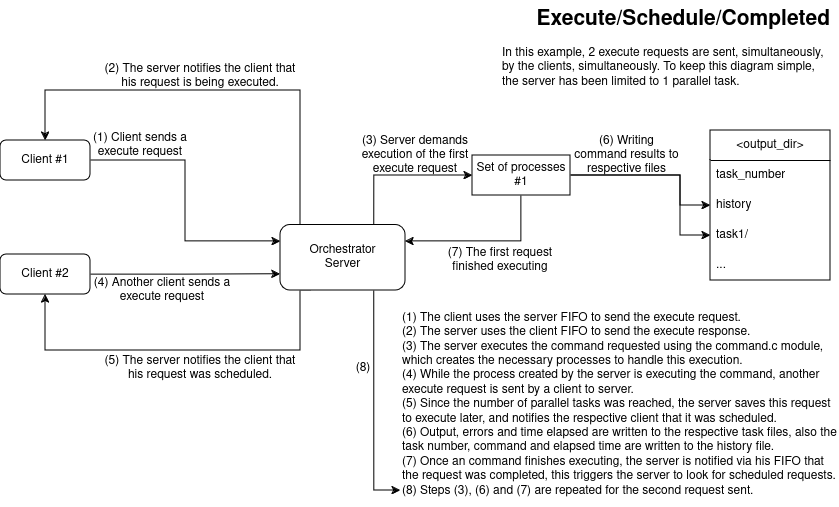
\includegraphics[width=\textwidth]{diagrams/execute_schedule.png}
                    \caption{Diagrama de Comunicação para Execução de Tarefas}
                    \label{fig:3.1}
                \end{figure}
        \subsection{Estado de Tarefas (\textit{status})}
            % \newgeometry{top=3cm,left=0.1cm,right=0.1cm,bottom=4cm}
            % \begin{figure}[!ht]
            %     \centering
            %     \includegraphics[scale=0.7]{diagrams/task_state.png}
            %     \caption{Diagrama de Comunicação para Estado de Tarefas}
            %     \label{fig:3.2}
            % \end{figure}
            % \loadgeometry{default}
        \subsection{Terminação do Servidor (\textit{kill})}
            % \newgeometry{top=3cm,left=0.1cm,right=0.1cm,bottom=4cm}
            % \begin{figure}[!ht]
            %     \centering
            %     \includegraphics[scale=0.7]{diagrams/server_termination.png}
            %     \caption{Diagrama de Comunicação para Terminação do Servidor}
            %     \label{fig:3.3}
            % \end{figure}
            % \loadgeometry{default}

\chapter{Argumentos da Interface de Linha de Comandos}
    \section{\textit{Orchestrator}}
    \section{\textit{Client}}

\chapter{Avaliação de Políticas de Escalonamento}
    No trabalho desenvolvido, foram implementadas três políticas de escalonamento de tarefas.
    Estas serão aprofundadas nas secções seguintes, assim como as suas avaliações práticas.
    Por favor consulte o anexo \nameref{anexo:2} para mais detalhes de como foi realizada
    a implementação destas políticas.

    \textcolor{red}{>> Atualizar a introdução da avaliação de políticas de escalonamento.}
    \section{\textbf{FCFS} - \textit{First Come First Served}}
        Nesta política, as tarefas são executadas por ordem de chegada, o que não é
        eficiente em termos de tempo de espera e execução. No entanto, é uma política
        simples e fácil de implementar.

        \textcolor{red}{>> Escrever sobre a avaliação prática desta política + Imagem}
    \section{\textbf{SJF} - \textit{Shortest Job First}}
        A política \textit{Shortest Job First} é uma política de escalonamento não preemptiva
        que seleciona a tarefa com o menor tempo de execução. Este tempo é passado como
        argumento na opção \textit{execute} do cliente e repesenta uma estimativa do tempo
        que a tarefa demorará a ser executada.

        Esta política é eficiente em termos de tempo de espera e execução, mas pode levar
        a situações de \textit{starvation}, que ocorrem quando tarefas com tempos de execução
        maiores são sempre adiadas, e, num caso extremo, quando surgem constantemente tarefas
        com tempos de execução menores, estas de maior duração nunca serão executadas.

        Existem várias maneiras de lidar com situações de \textit{starvation}, como, por exemplo,
        a criação de uma especificação de tempo máximo de espera para cada tarefa, ou a
        definição de um número máximo de tarefas que podem ser executadas antes de uma
        tarefa com tempo de execução maior. Outra solução seria a implementação de uma
        política de escalonamento preemptiva, permitindo esta a interrupção de tarefas em
        execução para dar lugar a tarefas com tempos de execução menores.

        \textcolor{red}{>> Escrever sobre a avaliação prática desta política + Imagem}
    \section{\textbf{PES} - \textit{Priority Escalonation Scheduling}}
        De forma a evitar situações de \textit{starvation}, foi implementada a política
        \textit{Priority Escalonation Scheduling}. Nesta, as tarefas são executadas
        de acordo com a sua prioridade, que é definida pelo cliente na opção \textit{execute},
        simliarmente como o tempo estimado que é passado como argumento na política \textit{SJF}.

        As tarefas com maior prioridade são executadas primeiro, evitando
        situações de \textit{starvation}. As prioridades ficam a critério do cliente,
        possibilitando uma maior versatilidade na execução de tarefas, permitindo ao cliente
        definir a prioridade adequada para cada tarefa que deseja executar. No entanto, esta
        flexibilidade não garante a eficiência da execução das tarefas, caso estas não sejam
        corretamente priorizadas.

        \textcolor{red}{>> Escrever sobre a avaliação prática desta política + Imagem}

\chapter{Testes Desenvolvidos}

%==========================================================================
% BEGIN CONCLUSÕES
%==========================================================================

\chapter{Conclusões}
    Após o desenvolvimento deste serviço, foram cumpridos todos
    os objetivos propostos no enunciado do trabalho, desde a implementação de
    uma interface de linha de comandos tanto para o servidor como para o cliente -
    que permite a execução de tarefas do utilizador de forma assíncrona com a
    possibilidade de encadeamento de programas com \textit{pipes} e a
    consulta do estado das tarefas -, assim como a implementação de um ficheiro
    \textit{log} para guardar as tarefas executadas, bem como a implementação de um
    sistema com várias políticas de escalonamento e a avaliação prática destas.
    Também foi desenvolvido um conjunto de testes que permitem verificar o correto
    funcionamento do serviço.

    Após a afirmação da possibilidade da terminação ou interrupção do servidor
    pelo professor regente, foi despertada a curiosidade de como o servidor
    poderia lidar com estas situações.

    Num estudo apronfundado desta unidade curricular, uma solução seria a
    implementação de um sistema de interrupções no servidor, o que permitiria
    a este lidar com situações de terminação ou interrupção de forma mais
    eficiente através da utlização dos sinais do sistema operativo para lidar com estas
    situações, evitando a perda de tarefas agendadas ou em execução.

    Para tal, seria necessário lidar com tarefas em execução, guardando
    o estado destas em memória, e permitindo a sua correta terminação
    ou interrupção, assim como para as tarefas em espera. Estas poderiam
    ser guardadas numa fila de espera, que seria consultada sempre que
    uma tarefa terminasse, permitindo a execução da próxima tarefa na
    fila.

    Em suma, o desenvolvimento deste serviço permitiu a aplicação prática
    dos conhecimentos adquiridos ao longo do semestre, assim como a
    exploração de novas funcionalidades e conceitos, que proporcionaram
    a implementação de um serviço robusto e versátil - serviço este que 
    propicia a execução de tarefas de forma assíncrona, com a possibilidade de
    encadeamento de programas e a consulta do estado das tarefas.

%==========================================================================
% END CONCLUSÕES
%==========================================================================

%==========================================================================
% BEGIN BIBLIOGRAFIA
%==========================================================================

%% Changes biblibography name
%% Portuguese babel default : “Bibliografia”
%% Personally I prefer “Referências”
% \renewcommand\bibname{Referências}

%% https://www.overleaf.com/learn/latex/bibliography_management_with_bibtex

% %% Add bibliografia to index
% \addcontentsline{toc}{chapter}{Bibliografia}

%==========================================================================
% END BIBLIOGRAFIA
%==========================================================================

%==========================================================================
% BEGIN LISTA DE SIGLAS E ACRÓNIMOS
%==========================================================================

%% Portuguese babel does not translate this environment
% \renewcommand{\nomname}{Lista de Siglas e Acrónimos}

%% Text that can be shown before acronyms list
% \renewcommand{\nompreamble}{
%     \textcolor{red}{
%         <<Apresentar uma lista com todas as siglas e acrónimos utilizados durante a realização do trabalho. O formato base para esta lista deverá ser da forma como abaixo se apresenta.>>
%     }
% }

%% acronyms
% \nomenclature[01]{\textbf{SO}}{Sistemas Operativos}

%% Show acronyms
% \printnomenclature

%==========================================================================
% END LISTA DE SIGLAS E ACRÓNIMOS
%==========================================================================

%==========================================================================
% BEGIN ANEXOS
%==========================================================================
%
%% Why \addchap, instead of \chapter?
%% \addchap has no numbering but appears in table of contents.
\addchap{Anexos}

    \addsec{
        \href{anexos/refman.pdf}{\small \textcolor{blue}{[I] Documentação do Código Desenvolvido}}
        \label{anexo:1}
    }

    \quad Para uma versão mais interativa da documentação do código desenvolvido, por favor consulte o
    ficheiro \textbf{\textit{doc/html/index.html}} localizado na diretoria raiz do projeto com o seu
    navegador de internet.

    \addsec{
        \href{anexos/example.pdf}{\small \textcolor{blue}{[II] Implementação das Políticas de Escalonamento}}
        \label{anexo:2}
    }

%==========================================================================
% END ANEXOS
%==========================================================================
\end{document}
